\documentclass[twocolumn]{article}
\usepackage{verbatim}
\usepackage{graphicx}
\usepackage{tabularx}
\usepackage{url}
\usepackage[htt]{hyphenat}

\newcommand{\naive}{Na\"\i ve}
\newcommand{\method}[1]{\texttt{#1()}}
\newcommand{\class}[1]{\texttt{#1}}
\newcommand{\param}[1]{\texttt{#1}}
\newcommand{\aicat}{\texttt{AI::Cat\-e\-gor\-i\-zer}}


\title{Streamlined Automatic Categorization of Mathematics Questions}

\author{
{\em Ken Williams}\\[1ex]
Web Engineering Group\\
The University of Sydney\\
Bldg J03, Sydney NSW 2006\\[1ex]
{\em kenw@ee.usyd.edu.au}
\and
{\em Rafael A. Calvo}\\[1ex]
Web Engineering Group\\
The University of Sydney\\
Bldg J03, Sydney NSW 2006\\[1ex]
{\em rafa@ee.usyd.edu.au}
\and
{\em David Bell}\\[1ex]
Web Engineering Group\\
The University of Sydney\\
Bldg J03, Sydney NSW 2006\\[1ex]
{\em dave@student.usyd.edu.au}
}

\begin{document}

\maketitle
\thispagestyle{empty}


\subsection*{\centering Abstract}
\noindent
{\it 
This paper describes a new approach to managing a stream of questions about 
mathematics by integrating a text categorization framework into a relational database 
management system. The corpus studied is based on unstructured submissions to a 
question-and-answer service in learning mathematics. The classification system has 
been tested using a K-Nearest Neighbour learner built into the framework. The 
performance results of the classifier are also discussed. The framework was integrated 
into a PostgreSQL database through the use of procedural trigger functions.
}

\paragraph{Keywords} 
XXX Need to write...



\section{Introduction}

Questions and answers services are becoming more common, spanning from standard 
customer relationship management to discussion forums in a particular discipline. In 
general, these online services are supported by domain experts who attempt to answer 
the questions posted. Since these experts often have a single domain of expertise it is 
very helpful if they have only to read questions that relate to this domain. This can be 
done by organizing the service in such a way that users are encouraged to post their 
question in the appropriate area. However this approach is not always successful as 
often the user will either ignore the organization or not know to which area their 
question belongs. 

These problems are common within a number of domains. Our test was performed on 
the Dr. Math questions and answers service for students and teachers. The issues 
discussed also apply to other similar systems such as customer relationship 
management (CRM) and e-learning systems in general. These systems can use an 
automatic text categorization framework to categorize the questions into the experts' 
area of interest, or into the appropriate customer support mailbox. 

The downside of an automatic categorization approach is that integrating such 
functionality into existing systems can be very complex, and often involves an in 
depth understanding of text categorization techniques.  Also, the content is normally 
stored in systems with a relational database in the backend, as is the case for most 
content and learning management systems. By building the categorizer into the 
database, the categorization framework\cite{williams:02} can be made invisible to the 
users and is thus more attractive to the average system administrator or application 
developer. Also, application developers, do not have to re-implement the 
classification software. They only need a machine learning professional to assist in 
training the classifier, and once trained it can then be reused in different applications. 

The applications of information retrieval have been well studied since the 1980s, as 
discussed by Salton \cite{salton:89,salton:91}, and many of these methodologies have been 
integrated into commercial database management systems that have free text search 
capabilities. However, this integration does not seem to have penetrated the text 
categorization domain.

Section 2 discusses the data set that was used to test the system. Section 3 of the 
paper discusses the text categorization framework and the extensions made to it, 
including the implementation within the database management system and the 
implementation of a "Learner" module. Section 4 discusses the quantitative results of 
the testing process and Section 5 concludes.

\section{Dr. Math Corpus}

For the evaluation of our system we have tested the performance of the
categorization system over a set of unstructured, informal documents
from the Ask Dr. Math
service.\footnote{\url{http://www.mathforum.org/dr.math/}} These
documents are mostly written by students as questions to a Mathematics
questions and answers service.  The documents vary greatly in length
from a single sentence to several paragraphs,
but all of them are relatively short. In addition to this most examples contain symbols 
and diagrams making linguistic analysis very difficult as well. The Dr. Math service 
has about 300 volunteers answering hundreds of questions a day. The volunteers have 
expertise in different areas of math and the site has won a number of awards for its 
useful service. 

The Dr. Math corpus we used contains 6632 documents and was split into a testing 
set of 1327 documents and a training set of 5305 documents.  There are 95 categories 
in the corpus. The average number of documents in each category is
107.15.  The most popular category, high school-level geometry,
contains 877 documents, and the least popular category,
elementary-level golden ratio, contains only 3 documents.  Each
document may be a member of more than one category, and the average
number of categories per document is 1.53.  Figure
\ref{cat-distribution} shows the distribution of categories throughout
the corpus.

\begin{figure}
\begin{verbatim}
Implicit Differentiation

Find the slope of the tangent at the point
(3,4) on the circle x^2 + y^2 = 25.

My answer: I guess we would need to put it
in the y = mx + b form. 

Thanks for any help,
Scott
\end{verbatim}
\caption{An example document from the Dr. Math corpus}
\end{figure}

Category names indicate an existing hierarchical ontology that was not used in our 
tests due to the relatively small number of documents available.

\begin{figure}
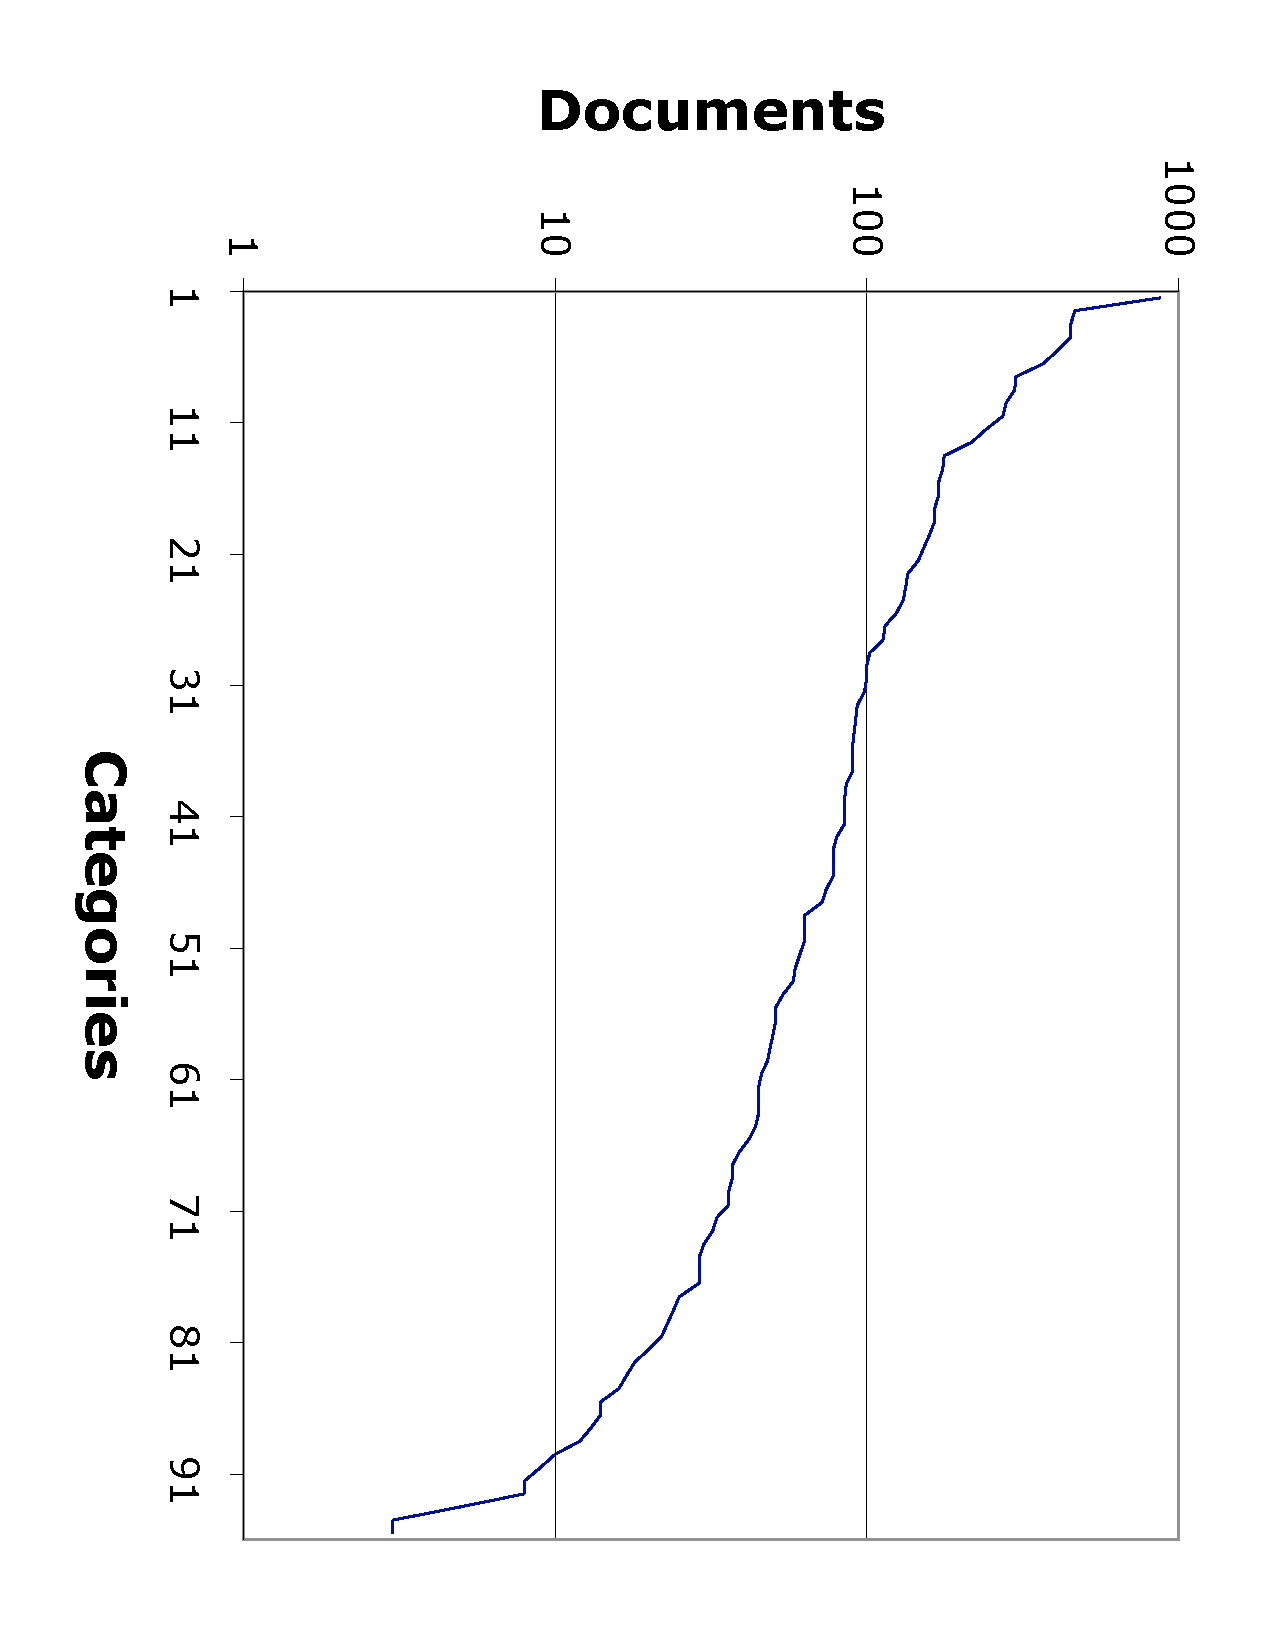
\includegraphics[angle=90,width=\linewidth]{cat-distribution}
\caption{Category distribution for the 95 Dr. Math categories}
\label{cat-distribution}
\end{figure}


\section{Categorization Framework}

Object Oriented Application Frameworks (OOAF) are software engineering artifacts 
that improve reusability of design and implementation \cite{fayad:97, fayad:99}.

The framework used in this project\footnote{\url{http://sourceforge.net/projects/ai-categorizer/}}
was designed to provide a 
consistent way to build document categorization systems.\cite{williams:02}  It allows the developer to 
focus on the quality of the more critical and complex modules by allowing reuse of 
common, simple base modules. In this project we extended the framework to fit our 
particular needs by adding a K-nearest neighbour `Learner' module. 

The framework already has implementations of support vector machines (SVM), 
\naive\ Bayes, and Decision Trees \cite{yang:99, sebastiani:02}. Other methods such 
as neural networks \cite{calvo:00, calvo:01} are being developed.

Also, an alternative Collection class was built to allow for the data to be read from a 
database instead of directly from file. These extensions are built by sub-classing two 
of the main classes in the framework. Class inheritance contributes to code reuse and 
quality. The framework also provides statistical analysis of experimental results, and 
produced the performance measures discussed in section 4. The framework is written 
in the Perl language. The architecture and language choice enabled us to easily build the 
framework into postgreSQL through postgreSQL's PL/Perl and PL/perlU support. 
This support allows the creation of procedural language functions through the use of 
the "Create Function" SQL command. Using this support and the pl/perlu language 
we were able to build a "launching" function that invoked the categorization 
framework on the document to be classified. This means that the only command 
necessary to categorize a document is a basic insert statement with a function call in 
place of a value for the category of the document.

\begin{figure}
\begin{verbatim}
 INSERT INTO documents
  (name, content, categories) 
 VALUES
  ('my name',
   'my content',
   categorize('my name',
              'my content',
              'documents'));
\end{verbatim}
\caption{Example document insertion statement with categorization}
\label{sql-insert}
\end{figure}

The statement in Figure \ref{sql-insert} can be further simplified through the creation of a pl/psql 
trigger function which fires automatically on insertion and passes the necessary values 
to the categorize function. 

If the categorization is to take place within a database, where often categorized 
documents are going to be appended to the learning set, a learning algorithm which has 
very little training overhead is ideal. This prevents the need to retrain a categorizer 
after each document insertion. K-nearest neighbour is one such learning algorithm. K-
nearest neighbour or KNN involves mapping each document to an n dimensional 
vector. When a document is to be classified it is also mapped to a vector and 
compared to the vectors of the documents in the learning set. The k documents which 
are closest (in vector space) to the document to be classified are kept for reference. 
These k documents are consulted and the most prevalent category amongst these 
documents is assigned to the new document. 

In the kNN learner module created, the comparison between vectors was made by 
normalizing each vector and 
finding their dot product. The dimension of each vector was, in this case, 
representative of the prevalence of a keyword in the document. This in effect gives a 
cosine of the two vectors being compared. 

The kNN module created has two customizable variables: threshold and k-value. The 
k-value governs how many neighbours are consulted to decide the category of the 
document. The threshold governs the confidence of the learner required to apply a 
category to a document. For example if a learner identifies 10 neighbours (i.e. k-value 
= 10) and finds 10 unique categories amongst those neighbours, the confidence for 
each category would be 10%. If the threshold is set to 0.15 the learner will not apply 
any category to the new document. Thus the threshold is a good control of precision 
within the classification system.

Since, the categorization performance is determined only by the classification 
framework, all these methods should behave as they do in standalone mode (outside 
the database). What the integration into the RDBMS does is to make the 
functionalities of the framework available as procedures in the SQL language.
Since relational databases can be designed using an object oriented methodology \cite{blaha:88,
rumbaugh:91}, by integrating it in this way, the classification task 
(and framework) can also be designed into larger OO systems.

\section{Method and Results}

The training set of the Dr Math corpus (5305 documents) was loaded into a database 
table named "documents". This table consisted of 3 columns, name, content and 
categories. The testing set was then inserted into the database, one document at a time 
using a statement similar to that in Figure \ref{sql-insert}. After each insert a SELECT query was 
run to extract the assigned categories. These categories were then compared to the 
actual categories of that document. Through this comparison the performance of the 
categorization in terms of recall  and performance  was measured. The precision and 
recall\footnote{Recall is the proportion of the target items that the
system selected, i.e. tp/(tp+fn).  Precision is the proportion of
selected items the system got right, i.e. tp/(tp+fp).} was then used
to calculate the F1 measure \cite{calvo:01,sebastiani:02}.

\begin{table}
\begin{tabular}{|r|r|r|r|r|}
\hline
k  & Threshold & Precision & Recall & $F_1$ \\ \hline
8  & 0.12 & 0.391 & 0.253 & 0.307 \\ \hline
8  & 0.15 & 0.524 & 0.238 & 0.327 \\ \hline
10 & 0.12 & 0.447 & 0.252 & 0.322 \\ \hline
10 & 0.15 & 0.617 & 0.228 & 0.333 \\ \hline
15 & 0.12 & 0.640 & 0.231 & 0.339 \\ \hline
15 & 0.15 & 0.740 & 0.211 & 0.328 \\ \hline
\end{tabular}
\caption{Macro averages against k-value and threshold}
\label{macro-results}
\end{table}

\begin{table}
\begin{tabular}{|r|r|r|r|r|}
\hline
k  & Threshold & Precision & Recall & $F_1$ \\ \hline
8  & 0.12 & 0.259 & 0.319 & 0.286 \\ \hline
8  & 0.15 & 0.296 & 0.291 & 0.293 \\ \hline
10 & 0.12 & 0.265 & 0.327 & 0.293 \\ \hline
10 & 0.15 & 0.339 & 0.282 & 0.308 \\ \hline
15 & 0.12 & 0.332 & 0.304 & 0.317 \\ \hline
15 & 0.15 & 0.397 & 0.260 & 0.314 \\ \hline
\end{tabular}
\caption{Micro averages against k-value and threshold}
\label{micro-results}
\end{table}

The results in Table \ref{macro-results} show that a Macro precision of 0.75 can be achieved for k=15 
and a threshold of 0.15, this is a good performance considering that this is noisy data 
and a small data set. Larger k or thresholds reduce the recall performance The recall 
was generally poor and this is probably due to the lack of training data and short, 
noisy and sometimes incoherent documents.
 
\begin{figure}
XXX Insert macro performance graph here...
% \includegraphics[width=\linewidth]{macro-perf-graph}
\caption{Macro performance averages}
\end{figure}
 

\section{Conclusion}

We have described a system that integrates a categorization framework into a 
relational database. The results show it is possible to integrate categorization 
techniques into the relational databases used by learning and content management 
systems.

A kNN classifier was built for the task of classifying postings in a discussion forum. 
The results show that a high precision can be reached even on  noisy data. The macro 
precision reached around 75%, however the recall was generally poor and this could be 
due to lack of training data and short, noisy and incoherent documents. The result 
achieved in this test however demonstrates that a KNN categorizer implemented 
within a database could have a high enough performance to be useful at classifying 
unstructured and informal data sets. 

\section*{Acknowledgements}

The authors gratefully acknowledge financial support from the Capital Markets 
Collaborative Research Centre and the University Of Sydney. The authors also 
acknowledge The Math Forum for giving permission to use and discuss their data. 

\bibliographystyle{plain}
\bibliography{TC-references}

\end{document}
